% 1977 年陕西卷参考题一：椭圆 x^2/a^2 + y^2/b^2 = 1 的内接矩形 ABCD，
% 长 AD=2x、宽 CD 为纵弦，x 轴标 ±a、y 轴标 ±b（按源卷第 6 页布局）
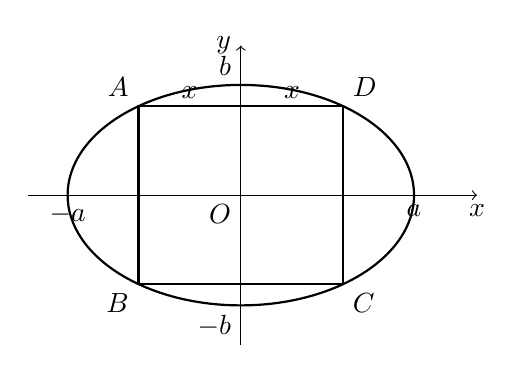
\begin{tikzpicture}[scale=1.0]
  \draw[->] (-2.7,0)--(3.0,0) node[below] {$x$};
  \draw[->] (0,-1.9)--(0,1.9) node[left] {$y$};
  \draw[thick] (0,0) ellipse (2.2 and 1.4);
  \draw[thick] (-1.3,-1.13) rectangle (1.3,1.13);
  \node[above left]  at (-1.3,1.13)  {$A$};
  \node[above right] at (1.3,1.13)   {$D$};
  \node[below left]  at (-1.3,-1.13) {$B$};
  \node[below right] at (1.3,-1.13)  {$C$};
  \node at (-0.65,1.3) {$x$};
  \node at (0.65,1.3)  {$x$};
  \node[below left]  at (0,0)     {$O$};
  \node[below]       at (-2.2,0)  {$-a$};
  \node[below]       at (2.2,0)   {$a$};
  \node[above left]  at (0,1.4)   {$b$};
  \node[below left]  at (0,-1.4)  {$-b$};
\end{tikzpicture}
